\section{Bounded Server Experiment}
\label{sec:server-experiment}

The experimental path was exercised under a two-CPU, 12-GiB Linux control group
(cgroup) on a shared server with strict policy
\texttt{\AFDExperimentReleasePolicyVersion}
(SHA-256 prefix \AFDExperimentReleasePolicyHashShort). The evidence package
retains the full digest. This bounded descriptive experiment
did not replace the
controlled release run in \cref{sec:evaluation}. Its estimands were
finite-corpus decision agreement, authorizing-parser acceptance, external
format or profile agreement, fidelity, fault and fuzz outcomes, and warm latency.
\Cref{tab:server-experiment-complete} reports selected retained outcomes and
their evidentiary limits.

\begingroup
\scriptsize
\setlength{\tabcolsep}{4pt}
\begin{longtable}{L{0.17\textwidth}L{0.39\textwidth}L{0.36\textwidth}}
\caption{Selected retained outcomes for the bounded server experiment. Counts
and proportions describe only the generated corpus and executed schedules.}
\label{tab:server-experiment-complete}\\
\toprule
Evidence area & Observed result & Evidence boundary \\
\midrule
\endfirsthead
\toprule
Evidence area & Observed result & Evidence boundary \\
\midrule
\endhead
\midrule
\multicolumn{3}{r}{Continued on next page}\\
\endfoot
\bottomrule
\endlastfoot
Provenance and validation &
Run \texttt{\AFDExperimentRunShort}. Corpus, fidelity, performance, and fuzz
evidence originated at \texttt{\AFDExperimentCorpusPerformanceCommit}.
external-validator and fault rechecks at
\texttt{\AFDExperimentAdapterFaultCommit}. Runner hardening occurred at
\texttt{\AFDExperimentRunnerCommit}, and packaging at
\texttt{\AFDExperimentEvidenceCommit} &
The campaign was not rerun under the final hardened runner.
All \AFDExperimentRustPassed{} Rust and \AFDExperimentResearchPassed{} research
tests passed. One fixture generator was ignored. Format, Clippy, package,
native-toolchain, \AFDExperimentBenchmarkSmokes{} benchmark-smoke, and
\AFDExperimentFuzzTargets{} fuzz-target checks passed \\
Corpus decisions &
\AFDExperimentCorpus{} generated records: S0 \(=\AFDExperimentStratumZero\),
S1 \(=\AFDExperimentStratumOne\), and inert S6
\(=\AFDExperimentStratumSix\). All 80 expected-clean evaluations delivered and
all 24 expected-block evaluations were blocked &
0/80 expected-clean records were withheld and 0/24 inert unsupported records
were delivered. No action, reason-family, or pipeline-state mismatch was
recorded \\
Closure and external validation &
\AFDExperimentExactStable{} exact and \AFDExperimentLossyClosure{} registered
semantic second-pass closures. \AFDExperimentDifferential{} record-level
external checks passed for \AFDExperimentUniqueOutputs{} unique output digests &
Each accepted record used at least two applicable tools drawn from ImageMagick
6.9.12-98, FFprobe/libavformat 6.1.1-3ubuntu5, and MediaInfo 24.01. These checks
established profile recognition or decodability, not canonical closure \\
Fidelity &
\AFDExperimentImageFidelity{} static, \AFDExperimentGifFidelity{} GIF,
\AFDExperimentAudioFidelity{} audio, \AFDExperimentMpFourFidelity{} MP4,
\AFDExperimentWebmFidelity{} source-WebM. \AFDExperimentFidelityPassed{} overall &
Audio duration drift \AFDExperimentAudioDurationDrift\% with per-record mean
scale-invariant signal-to-distortion ratio (SI-SDR)
\AFDExperimentAudioSiSdr{} dB. Source-WebM structural similarity index (SSIM)
\AFDExperimentWebmSsim{} with drift
\(\leq\AFDExperimentWebmDurationDrift\%\). No failure was waived \\
Fault and fuzz campaigns &
\AFDExperimentFaultCampaigns{} selected single-test fault checks passed.
Seven fuzz targets each received one seeded run with a requested 30-second
budget, for 210 requested target-seconds &
\AFDExperimentFuzzExecutions{} iterations produced no recorded crash, sanitizer
finding, timeout, or crash artifact. The protocol requested three one-hour
repetitions per target \\
Performance &
\AFDExperimentPerformanceObservations{} observations =
\AFDExperimentColdObservations{} cold + \AFDExperimentWarmObservations{} warm.
Cold median/p95 \AFDExperimentColdMedian{}/\AFDExperimentColdPninetyfive{} ms.
Warm \AFDExperimentWarmMedian{}/\AFDExperimentWarmPninetyfive{} ms. Peak RSS
\AFDExperimentPeakRss{} KiB &
Warm observations equal 104 records \(\times\) 5 repetitions \(\times\) 3
sessions and are not independent samples. Warm mean
\AFDExperimentWarmMean{} ms/call corresponds to
\AFDExperimentSequentialRate{} sequential calls/s for this order and host.
No bootstrap interval was produced.
Warm median/p95: unsupported
\AFDExperimentUnsupportedMedian{}/\AFDExperimentUnsupportedPninetyfive, raster
\AFDExperimentRasterMedian{}/\AFDExperimentRasterPninetyfive, GIF
\AFDExperimentGifMedian{}/\AFDExperimentGifPninetyfive, audio
\AFDExperimentAudioMedian{}/\AFDExperimentAudioPninetyfive, video
\AFDExperimentVideoMedian{}/\AFDExperimentVideoPninetyfive{} ms \\
Mechanism ablation &
Three conditions were prespecified but not executed in this bounded package &
No paired transition or mechanism-contribution claim is authorized \\
\(G_{\mathrm{sci}}\) and release candidate &
Ineligible &
S2--S5 and S7 absent. Required public-benign coverage absent. Shortened fuzz
and performance schedules. Thirty-three other containers active on the host.
External tools were mutable. No append-only publication. Fidelity gate
failed \\
\end{longtable}
\endgroup

\begin{figure}[tbp]
\centering
\definecolor{AFDPass}{RGB}{28,125,117}
\definecolor{AFDFail}{RGB}{190,77,62}
\definecolor{AFDMedian}{RGB}{36,86,150}
\definecolor{AFDPninetyfive}{RGB}{214,129,45}

\begin{minipage}[t]{0.48\textwidth}
\centering
\textbf{\small (a) Fidelity-gate outcomes}

\vspace{3pt}
\resizebox{\linewidth}{!}{%
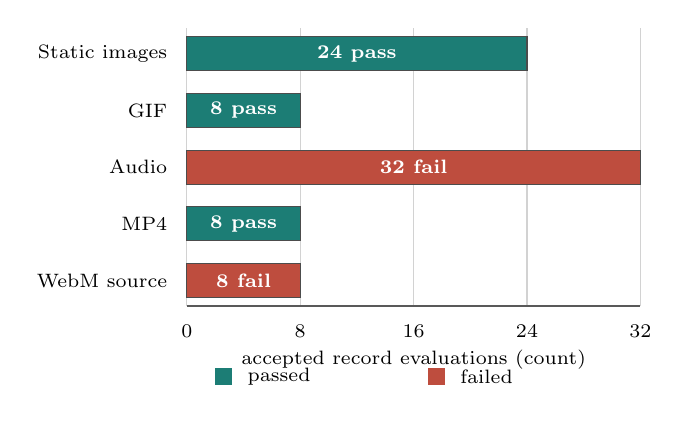
\begin{tikzpicture}[x=0.18cm,y=0.72cm,font=\scriptsize]
  \foreach \x in {0,8,16,24,32} {
    \draw[gray!35] (\x,0.55) -- (\x,5.45);
    \node[anchor=north] at (\x,0.38) {\x};
  }
  \node[anchor=east] at (-0.7,5) {Static images};
  \node[anchor=east] at (-0.7,4) {GIF};
  \node[anchor=east] at (-0.7,3) {Audio};
  \node[anchor=east] at (-0.7,2) {MP4};
  \node[anchor=east] at (-0.7,1) {WebM source};

  \filldraw[fill=AFDPass,draw=black!70] (0,4.70) rectangle (24,5.30);
  \node[text=white,font=\scriptsize\bfseries] at (12,5) {24 pass};
  \filldraw[fill=AFDPass,draw=black!70] (0,3.70) rectangle (8,4.30);
  \node[text=white,font=\scriptsize\bfseries] at (4,4) {8 pass};
  \filldraw[fill=AFDFail,draw=black!70] (0,2.70) rectangle (32,3.30);
  \node[text=white,font=\scriptsize\bfseries] at (16,3) {32 fail};
  \filldraw[fill=AFDPass,draw=black!70] (0,1.70) rectangle (8,2.30);
  \node[text=white,font=\scriptsize\bfseries] at (4,2) {8 pass};
  \filldraw[fill=AFDFail,draw=black!70] (0,0.70) rectangle (8,1.30);
  \node[text=white,font=\scriptsize\bfseries] at (4,1) {8 fail};

  \draw[black!65] (0,0.55) -- (32,0.55);
  \node[anchor=north] at (16,-0.05) {accepted record evaluations (count)};
  \fill[AFDPass] (2,-0.85) rectangle (3.2,-0.55);
  \node[anchor=west] at (3.6,-0.70) {passed};
  \fill[AFDFail] (17,-0.85) rectangle (18.2,-0.55);
  \node[anchor=west] at (18.6,-0.70) {failed};
\end{tikzpicture}%
}
\end{minipage}
\hfill
\begin{minipage}[t]{0.48\textwidth}
\centering
\textbf{\small (b) Warm latency by execution class}

\vspace{3pt}
\resizebox{\linewidth}{!}{%
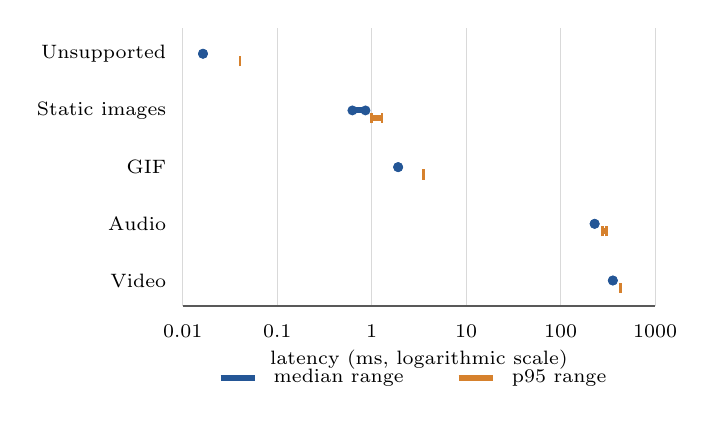
\begin{tikzpicture}[x=0.48cm,y=0.72cm,font=\scriptsize]
  % Maps latency t in milliseconds onto a log10 axis from 0.01 to 1000 ms.
  \newcommand{\latencyrange}[6]{%
    \node[anchor=east] at (-0.18,#1) {#2};
    \pgfmathsetmacro{\medianlo}{2.5*(ln(#3)/ln(10)+2)}
    \pgfmathsetmacro{\medianhi}{2.5*(ln(#4)/ln(10)+2)}
    \pgfmathsetmacro{\pninetyfivelo}{2.5*(ln(#5)/ln(10)+2)}
    \pgfmathsetmacro{\pninetyfivehi}{2.5*(ln(#6)/ln(10)+2)}
    \draw[AFDMedian,line width=2.2pt] (\medianlo,#1) -- (\medianhi,#1);
    \fill[AFDMedian] (\medianlo,#1) circle[radius=1.8pt];
    \fill[AFDMedian] (\medianhi,#1) circle[radius=1.8pt];
    \draw[AFDPninetyfive,line width=2.2pt]
      (\pninetyfivelo,{#1-0.13}) -- (\pninetyfivehi,{#1-0.13});
    \draw[AFDPninetyfive,line width=1pt]
      (\pninetyfivelo,{#1-0.22}) -- (\pninetyfivelo,{#1-0.04});
    \draw[AFDPninetyfive,line width=1pt]
      (\pninetyfivehi,{#1-0.22}) -- (\pninetyfivehi,{#1-0.04});
  }
  \foreach \x/\lab in {0/{0.01},2.5/{0.1},5/{1},7.5/{10},10/{100},12.5/{1000}} {
    \draw[gray!30] (\x,0.55) -- (\x,5.45);
    \node[anchor=north] at (\x,0.38) {\lab};
  }

  \latencyrange{5}{Unsupported}{0.016}{0.016}{0.040}{0.040}
  \latencyrange{4}{Static images}{0.625}{0.860}{0.998}{1.284}
  \latencyrange{3}{GIF}{1.906}{1.906}{3.561}{3.561}
  \latencyrange{2}{Audio}{228.799}{228.975}{279.765}{304.897}
  \latencyrange{1}{Video}{356.371}{357.113}{432.328}{433.799}

  \draw[black!65] (0,0.55) -- (12.5,0.55);
  \node[anchor=north] at (6.25,-0.05) {latency (ms, logarithmic scale)};
  \draw[AFDMedian,line width=2.2pt] (1.0,-0.72) -- (1.9,-0.72);
  \node[anchor=west] at (2.15,-0.72) {median range};
  \draw[AFDPninetyfive,line width=2.2pt] (7.3,-0.72) -- (8.2,-0.72);
  \node[anchor=west] at (8.45,-0.72) {p95 range};
\end{tikzpicture}%
}
\end{minipage}

\caption{Fidelity outcomes by source or metric group and warm latency by
execution class. Panel (a) reports 80 accepted record-level evaluations
representing 40 unique output digests. Panel (b) reports the range of profile
medians and p95 values within each execution class across 1,560 repeated warm
calls, equal to 104 records times five repetitions times three shortened
sessions. The logarithmic axis separates immediate rejection, in-process
reconstruction, and external codec paths. The observations describe this
generated corpus and host only.}
\label{fig:server-experiment-profile-results}
\end{figure}


Fidelity used the versioned policy
\texttt{\AFDExperimentFidelityPolicyVersion}. Its SHA-256 digest begins with
\AFDExperimentFidelityPolicyHashShort. Static images required equal dimensions and
peak signal-to-noise ratio (PSNR) \(\geq40\) dB. Animated images additionally
required equal canvas and frame count, timing drift \(\leq2\%\), and frame PSNR
\(\geq40\) dB. Video required equal dimensions, duration drift \(\leq2\%\), and
SSIM \(\geq0.90\). Audio required equal channels, duration drift \(\leq2\%\),
and SI-SDR \(\geq20\) dB. Audio failed only the duration threshold.
Source-WebM inputs, semantically emitted as MP4, failed only SSIM.

The full policy matched the fixture-derived expected action, reason family, and
pipeline state for all 104 records. The 80 accepted record-level evaluations,
representing 40 unique emitted-byte digests, satisfied exact or registered
semantic second-pass closure and passed at least two applicable external
format/profile checks. Eleven selected single-test fault checks passed. No
publication-invariant violation was observed in those 11 executions, and no
crash or recorded fuzz failure occurred during the shortened schedule. These
are finite-schedule observations, not population failure-rate estimates.

\Cref{fig:server-experiment-profile-results} shows two operational limitations.
Security acceptance did not imply usability acceptance: all 32 audio and all 8
source-WebM evaluations failed their fidelity profiles, while 24 static-image,
8 GIF, and 8 MP4 evaluations passed. Latency differed by execution path.
Unsupported active inputs terminated in tens of microseconds, static images
completed below 1 ms at the median, GIF in 1.906 ms, audio near 229 ms, and
video near 357 ms. The mixed-corpus warm mean was
\AFDExperimentWarmMean{} ms/call, corresponding to
\AFDExperimentSequentialRate{} sequential calls/s for this order and host. This
is a service rate, not concurrent capacity or deployment throughput.

The action result is a generated-fixture and policy consistency check, not
independent ground-truth validation or evidence of source diversity. External
format/profile checks corroborate emitted outputs but do not independently
validate expected decisions. The experiment therefore supports bounded
record-level conformance observations and separately characterizes fidelity and
finite-schedule latency for the tested records. The latency figure uses 1,560
repeated warm calls, not independent samples. The shortened schedule supplies
neither the prespecified bootstrap intervals nor a controlled RQ3 cost result.
The experiment does not isolate the
prescan, supplied type evidence, or reconstruction floor because no paired
ablation stream was retained. The absent strata, controlled host,
prespecified schedule, immutable external tools, and ablation results keep
\cref{eq:scientific-gate} false and preclude broader efficacy or mechanism
claims.

\subsection{Public-source compatibility and readiness rehearsals}
\label{sec:public-source-rehearsals}

\Cref{tab:public-source-evidence-status} separates the retained observations
from the authority they provide. The sequence increases operational readiness
for external review but satisfies neither corpus admission nor
\(G_{\mathrm{sci}}\).

\begin{table}[H]
\centering
\caption{Evidence status of the public-source compatibility and readiness
rehearsals. Counts are retained observations. The evidence boundary states the
maximum supported interpretation for each stage.}
\label{tab:public-source-evidence-status}
\begingroup
\scriptsize
\setlength{\tabcolsep}{3.2pt}
\begin{tabularx}{\textwidth}{L{0.17\textwidth}L{0.43\textwidth}Y}
\toprule
Stage & Retained evidence & Evidence boundary \\
\midrule
Public-benign pilot &
At runner commit \texttt{\AFDPublicPilotRunnerCommit},
\AFDPublicPilotAccepted{} expected-benign records were accepted:
\AFDPublicPilotExactStable{} byte-idempotent and
\AFDPublicPilotLossyClosure{} registered lossy closures. Evidence commit:
\texttt{\AFDPublicPilotEvidenceCommit} &
No expected-block record was present, so false acceptance was not estimable.
This is finite compatibility evidence only \\
Candidate inventory &
\AFDWikimediaCandidates{} Wikimedia Commons and
\AFDInternetArchiveCandidates{} Internet Archive candidates yielded
\AFDCombinedCandidates{} distinct SHA-256 identities totaling
\AFDCombinedCandidateBytes{} bytes. Evidence commit:
\texttt{\AFDCandidateEvidenceCommit} &
The raw shortfall for \AFDRequiredPublicSourceSlots{} planned public-source
slots fell to zero, but the objects remained candidates rather than audited or
admitted corpus records \\
Mechanical packet &
Commit \texttt{\AFDAuditPacketCommit} verified
\AFDMechanicallyVerifiedCandidates{} byte identities and retained
\AFDExactInspectionOutputs{} exact inspection outputs; encoder metadata was
observed for \AFDEncoderMetadataObserved{} candidates &
No provenance, license, diversity, or encoder label was independently
reviewed. All \AFDPendingReviewCandidates{} candidates remained pending and
the reviewed-slot deficit was \AFDReviewedSlotDeficit{} \\
Review and selection &
The worklist required \AFDReviewApprovalsRequired{} matching detached Ed25519
approvals from different reviewer clusters. At selection commit
\texttt{\AFDSelectionCommit}, all \AFDSelectionProfileStrata{} cells lacked
approved sources and \AFDSelectedPublicSources{}/\AFDRequiredPublicSourceSlots{}
sources were selected &
No registry, controlled key, signed decision, consensus approval, S0/S1
assignment, full-file admission, or frozen manifest existed; selection failed
closed \\
Offline handoff &
Commit \texttt{\AFDReviewHandoffCommit} produced a byte-complete,
write-disabled packet with \AFDReviewHandoffDecisionInputs{} source decision
contexts, \AFDReviewHandoffProviderEvidence{} provider-evidence references,
\AFDExactInspectionOutputs{} inspection outputs, and a frozen Ed25519
author/sign tool. The \AFDReviewHandoffArchiveBytes{}-byte archive has SHA-256
prefix \texttt{\AFDReviewHandoffArchiveHashShort}; all
\AFDReviewHandoffResearchTests{} research tests passed. Evidence commit:
\texttt{\AFDReviewHandoffEvidenceCommit} &
The packet contains \AFDReviewHandoffPrivateKeys{} private keys,
\AFDReviewHandoffDecisions{} decisions, and
\AFDReviewHandoffSignatures{} signatures. It makes independent review
executable, not completed or approved \\
\bottomrule
\end{tabularx}
\endgroup
\end{table}
